\documentclass[10pt]{article}
\usepackage{icmlko}

\icmlmeta{IP 파운데이션 월드모델}{16}{가격은 허들이 아니다}{두 도메인이 독립적으로 같은 답을 냈다 --- 그리고 누출을 고치자 게임이 되살아났다}

\begin{document}

\twocolumn[
\icmlheader

\begin{abstract}
노트 15는 게임의 굿즈 규모 축(DLC 수)이 누출임을 밝히고 그 자리를 비웠다. 이 노트는
누출 없는 대체 측정을 찾고, 그 과정에서 두 번째 축도 무너뜨린다. 30일 창 라벨을
기준으로 여섯 개 후보를 훑었다. \textbf{가격이 가장 강한데(r=$+$0.310) 방향이
틀렸다} --- 무료 게임의 출시 반응이 유료보다 \emph{작다}(표준화 평균 $-$0.244 대
$+$0.051). 허들 해석이 맞다면 반대여야 한다. 아이돌에서 앨범 가격이 허들이 아니라
규모 신호였던 것(노트 9)과 같은 결과이며, \textbf{두 도메인이 독립적으로 같은 답을
냈다.} ``입장 허들''은 가격으로 잴 수 없다. 굿즈 규모의 대체 측정으로는 Steam
기능 수(도전 과제·트레이딩 카드·워크샵)를 골랐다 --- 출시 시점 확정, DLC와 거의
무상관(r=$+$0.084), 창 라벨과 $+$0.224. 재배선 결과 \textbf{게임 도메인 내부 성적이
$-$0.0098에서 $-$0.0332로 3.4배 개선됐다.} 누출 축을 빼고 옳은 측정을 넣으니 실제로
더 잘 작동한다. 공유 슬롯도 둘로 복구되고 전이 넷이 유지된다. 다만 노트 15의 배율
가설에 대한 답은 부정적이다 --- 대상 도메인 라벨 k개로 배율을 보정해도 상수와의
격차가 넓어지지 않는다(k=0에서 30까지).
\end{abstract}
]

\section{대체 측정을 찾는다}

노트 15는 게임의 굿즈 규모를 비운 채 끝났다. 그 자리를 채울 후보를 30일 창 라벨을
기준으로 훑었다. 좋은 후보의 조건은 둘이다 --- 창 라벨을 설명해야 하고, 경과
시간과 상관이 없어야 한다(있으면 누출 의심).

\begin{figure}[t]
\centering
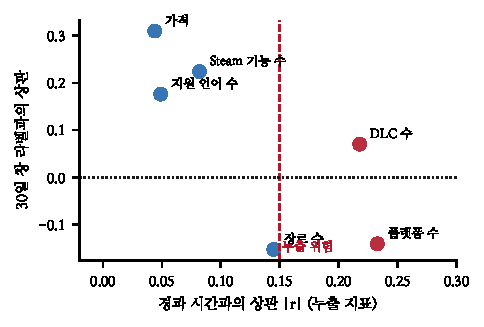
\includegraphics[width=\columnwidth]{figs/proxy.pdf}
\caption{후보 훑기. 오른쪽으로 갈수록 누출 위험이 크고 위로 갈수록 설명력이 크다.
왼쪽 위가 좋다.}
\end{figure}

\begin{table}[t]
\centering\tsize
\caption{굿즈·허들 후보(n=434, 30일 창 라벨).}
\begin{tabular}{lrr}
\toprule
후보 & 경과 시간과 r & 창 라벨과 r \\
\midrule
가격 & $-$0.044 & \textbf{$+$0.310} \\
Steam 기능 수 & $+$0.082 & $+$0.224 \\
지원 언어 수 & $+$0.049 & $+$0.176 \\
장르 수 & $-$0.145 & $-$0.153 \\
플랫폼 수 & $+$0.233 & $-$0.141 \\
DLC 수 (노트 15의 누출) & $+$0.218 & $+$0.070 \\
\bottomrule
\end{tabular}
\end{table}

가격이 압도적으로 강하다. 누출 위험도 없다(경과 시간과 $-$0.044). 그런데 가격은
이미 ``입장 허들'' 자리에 있다. 그래서 그 자리가 맞는지부터 확인했다.

\section{입장 허들이 무너진다}

게임 도메인의 입장 허들은 두 부분으로 만들었다 --- 무료 여부가 주 신호이고,
유료 구간 안에서는 가격이 보조다. 무료면 허들 0이라는 전제다.

\begin{figure}[t]
\centering

\includegraphics[width=\columnwidth]{figs/price.pdf}
\caption{무료 게임의 출시 반응이 유료보다 작다. 허들 해석의 예측과 반대다.}
\end{figure}

\begin{table}[t]
\centering\tsize
\caption{가격과 출시 30일 반응(표준화, 탈추세).}
\begin{tabular}{lr}
\toprule
무료 게임(75건) 평균 반응 & $-$0.244 \\
유료 게임(359건) 평균 반응 & $+$0.051 \\
무료 여부와 반응의 상관 & $-$0.111 \\
\midrule
유료 구간 내 가격(log)과 반응 & $+$0.303 \\
\bottomrule
\end{tabular}
\end{table}

두 가정이 모두 틀렸다. 무료 게임의 반응이 \emph{작고}, 유료 구간 안에서 비쌀수록
반응이 \emph{크다}. 허들이라면 둘 다 반대여야 한다.

읽는 방법은 하나다. 가격은 치르는 값이 아니라 \textbf{만든 규모를 알리는 신호}다.
비싼 게임은 큰 제작비를 뜻하고, 무료 게임은 대체로 작은 제작이다.

\claimx{게임 도메인에서도 가격은 입장 허들이 아니라 규모 신호다. 아이돌에서 앨범
가격이 그랬던 것(노트 9)과 같으며, 두 도메인이 독립적으로 같은 답을 냈다.
``입장 허들'' 축은 가격으로 측정할 수 없다.}{가격을 통제한 뒤에도 접근 난이도
지표(지역 잠금, 사양 요구, 사전 가입 절차)가 반응과 음의 관계를 가지면, 축은
살아 있고 가격이 잘못된 측정이었을 뿐이다.}

이것은 축 하나를 잃는 손실이지만, 두 도메인에서 같은 방식으로 실패했다는 점이
오히려 정보다. ``닿는 데 무엇을 치르는가''는 실재하는 축일 수 있으나 \emph{가격은
그것을 재지 않는다}. 가격은 ``닿으면 무엇을 얻는가''의 다른 얼굴이다.

\section{Steam 기능 수로 굿즈 규모를 되살린다}

가격을 허들에서 뺐으니 굿즈 규모의 측정이 남는다. Steam 기능 수 --- 도전 과제,
트레이딩 카드, 워크샵 지원, 클라우드 저장 등 --- 를 골랐다.

\begin{itemize}[leftmargin=1.1em,itemsep=0.15em]
\item \textbf{출시 시점 확정} --- 스토어 기능은 출시 때 붙는다.
\item \textbf{DLC와 거의 무상관} (r=$+$0.084) --- 누출된 축과 독립이다.
\item \textbf{경과 시간과 약함} (r=$+$0.082) --- 누적 신호가 아니다.
\item \textbf{창 라벨과 $+$0.224} --- DLC(+0.070)보다 세 배 강하다.
\item 의미도 맞다 --- ``닿으면 무엇을 얻는가''.
\end{itemize}

재배선하고 전부 다시 쟀다.

\begin{table}[t]
\centering\tsize
\caption{게임 축 재배선 전후.}
\begin{tabular}{lrr}
\toprule
& 노트 15 (굿즈 비움) & 이 노트 \\
\midrule
게임 도메인 내부 & $-$0.0098 & \textbf{$-$0.0332} \\
게임 굿즈 규모 계수 & --- & $+$0.263 \\
공유 슬롯 수 & 1 & \textbf{2} \\
\bottomrule
\end{tabular}
\end{table}

\textbf{게임 도메인 내부 성적이 3.4배 개선됐다.} 누출된 축을 빼고 옳은 측정을
넣으니 실제로 더 잘 작동한다 --- 누출은 성능을 부풀리는 것이 아니라 갉아먹고
있었다.

\begin{table}[t]
\centering\tsize
\caption{재배선 후 여섯 방향 전이. 순열 3,000회.}
\begin{tabular}{lrl}
\toprule
방향 & 차이 & p \\
\midrule
팝업 $\to$ 아이돌 & $-$0.0744 & \textbf{0.0013} \\
게임 $\to$ 아이돌 & $-$0.0715 & \textbf{$<$0.0001} \\
아이돌 $\to$ 팝업 & $-$0.0467 & \textbf{0.0480} \\
게임 $\to$ 팝업 & $-$0.0458 & \textbf{0.0003} \\
팝업 $\to$ 게임 & $-$0.0239 & 0.0837 \\
아이돌 $\to$ 게임 & $+$0.0104 & 0.4957 \\
\bottomrule
\end{tabular}
\end{table}

넷이 유지되고, 게임 $\to$ 아이돌은 $-$0.0455에서 $-$0.0715로 강해졌다. 계수도
세 도메인 모두 양수다(굿즈 규모 $+$0.211 / $+$0.435 / $+$0.263).

\section{그러나 배율 가설은 부정된다}

노트 15는 공유 헤드가 쌍 전이보다 못한 이유를 계수 크기 차이로 지목하고, 도메인별
배율 항을 두면 유의성이 돌아와야 한다는 반증 조건을 적었다.

배율은 대상 도메인 라벨이 있어야 추정된다. 그래서 질문을 바꿨다 --- \emph{몇 개면
되는가.} 두 도메인으로 공유 방향을 배우고, 대상 도메인 라벨 k개만 보고 배율과
절편을 맞춘 뒤 나머지에서 잰다. 상수 기준도 같은 k개만 본다.

\begin{figure}[t]
\centering
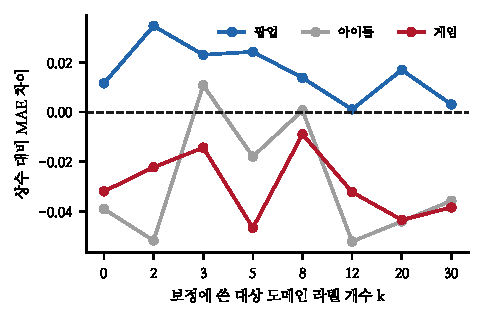
\includegraphics[width=\columnwidth]{figs/fewshot.pdf}
\caption{보정에 쓴 라벨 개수에 따른 상수 대비 성적. 0 아래가 이기는 것이다.
격차가 k에 따라 넓어지지 않는다.}
\end{figure}

\begin{table}[t]
\centering\tsize
\caption{소수 예시 보정. 40회 반복 평균, 상수 대비 차이.}
\begin{tabular}{lrrrr}
\toprule
k & 0 & 5 & 12 & 30 \\
\midrule
게임   & $-$0.0319 & $-$0.0466 & $-$0.0322 & $-$0.0384 \\
아이돌 & $-$0.0390 & $-$0.0179 & $-$0.0521 & $-$0.0357 \\
팝업   & $+$0.0116 & $+$0.0243 & $+$0.0011 & $+$0.0031 \\
\bottomrule
\end{tabular}
\end{table}

k=0이 이미 최선에 가깝다. 라벨을 더 주면 모델도 좋아지지만 상수도 같이 좋아지므로
격차가 넓어지지 않는다.

\paragraph{첫 시도는 파탄났다}
처음에는 자유 최소제곱으로 배율과 절편을 맞췄다. k=2에서 팝업 MAE가 8.97까지
올라갔다 --- 보정하지 않은 값이 0.77인데. 두 점에 직선을 맞추면 기울기가 폭주한다.
예측과 라벨이 같은 눈금에 있으므로 기울기의 사전값은 1이며, 수축 계수
$k/(k{+}\lambda)$로 자료 쪽에 서서히 옮겨가도록 고쳤다.

\claimx{도메인별 배율 보정으로는 공유 헤드의 열세가 해소되지 않는다. 노트 15의
계수 크기 가설은 실용적 해법을 주지 못한다.}{배율이 아니라 방향까지 도메인별로
풀었을 때(즉 공유 헤드를 포기했을 때) 격차가 커지면, 문제는 눈금이 아니라
공유 자체다.}

\section{한계}

\begin{itemize}[leftmargin=1.1em,itemsep=0.15em]
\item 신경망의 시드 분산이 크다. 같은 설정에서 팝업 예측 MAE가 시드 수에 따라
      0.7357에서 0.7733까지 움직였다. 표본이 작아 생기는 문제이며, 보고한
      파운데이션 수치는 이 분산 안에 있다.
\item Steam 기능 수가 출시 시점에 확정된다는 것은 논증이다. 기능이 나중에 추가되는
      경우(워크샵 지원 후속 패치)를 배제하지 못했다.
\item 입장 허들 축은 이제 세 도메인 모두에서 비어 있다. 대체 측정을 못 찾으면
      다섯 축 중 하나를 영구히 잃는다.
\item 30일 창 검정은 게임에서만 했다. 팝업·아이돌의 굿즈 축이 누출이 아니라는
      것은 여전히 논증이다.
\end{itemize}

\section{다음}

\begin{enumerate}[leftmargin=1.3em,itemsep=0.15em]
\item 입장 허들의 진짜 측정 --- 접근 난이도(예약 경쟁, 지역 제한, 사양 요구)를
      가격과 분리해 수집한다.
\item 팝업·아이돌 굿즈 축의 누출 검정 --- 게임에서 쓴 30일 창 방식을 옮긴다.
\item 공유 헤드를 포기한 대조군 --- 배율 가설의 마지막 반증 조건.
\item 신경망 시드 분산 정량화 --- 보고 수치에 구간을 붙인다.
\end{enumerate}

\vspace{0.6em}
\hrule height 0.3pt
\vspace{0.5em}
{\footnotesize
\textbf{참고문헌}\\[0.3em]
Kaufman, S., Rosset, S., Perlich, C. (2012). Leakage in data mining.
\emph{ACM TKDD}, 6(4), 1--21.\\[0.15em]
Efron, B., Morris, C. (1975). Data analysis using Stein's estimator and its
generalizations. \emph{JASA}, 70(350), 311--319.\\[0.15em]
Standley, T. et al. (2020). Which tasks should be learned together in multi-task
learning? \emph{ICML 2020}, 9120--9132.\\[0.15em]
Ben-David, S. et al. (2010). A theory of learning from different domains.
\emph{Machine Learning}, 79(1--2), 151--175.
}

\end{document}
